\section{Results}\label{sec:results}

All numbers are computed on the test questions by scripts from the saved outputs; counts are over (system, question) pairs unless stated otherwise. Table~\ref{tab:overview} summarises every tool at every tier and Table~\ref{tab:hypotheses} the pre-registered hypotheses; analyses that were not pre-registered are marked \emph{post hoc}.

% ICDE overview table; all numbers are macros from numbers.tex (generated by src/make_numbers.py)
\begin{table*}[t]
\centering\footnotesize
\caption{Overview on the test pairs. \emph{Certified}: EX-correct pairs ($n=\V{nExc}$) with a witness that our certifier accepts at each tier (re-certified for SpotIt/SpotIt+); \emph{Claimed}: pairs the released results classify as non-equivalent. \emph{Recall}: share of known positives ($n=\V{nExi}$) with a witness. \emph{Attribution}: random sample of 100 witnesses per tool at the tier given in parentheses; \emph{Est.\ meaningful}: certified count $\times$ meaningful share (95\,\% CI). --: not applicable or not sampled.}\label{tab:overview}
\setlength{\tabcolsep}{4pt}
\begin{tabular}{@{}l r rrrrr rr rrl@{}}
\toprule
& & \multicolumn{5}{c}{Certified EX-correct pairs} & \multicolumn{2}{c}{Recall (\%)} & \multicolumn{3}{c}{Attribution of witnesses}\\
\cmidrule(lr){3-7}\cmidrule(lr){8-9}\cmidrule(l){10-12}
Tool & Claimed & $\mathcal A_0$ & $\mathcal A_{1f}$ & $\mathcal A_2$ & $\mathcal A_{Rq}$ & $\mathcal A_R$ & $\mathcal A_{1f}$ & $\mathcal A_R$ & Impl.\,\% (tier) & Mean.\,\% & Est.\ meaningful [CI]\\
\midrule
SpotIt & \V{nSIClaims} & \V{nSILzero} & \V{nSILonef} & \V{nSILtwo} & \V{nSIAtRq} & \V{nSIAtR} & \V{rSI}$^{*}$ & -- & \V{pSIImpl} ($\mathcal A_0$) & \V{pSIMeaningful} & \V{estSIMeaningful} \V{estSIMeaningfulCI}\\
SpotIt+ & \V{nSIPClaims} & \V{nSIPLzero} & \V{nSIPLonef} & \V{nSIPLtwo} & \V{nSIPAtRq} & \V{nSIPAtR} & -- & -- & \V{pSIPImpl} ($\mathcal A_0$) & \V{pSIPMeaningful} & \V{estSIPMeaningful} \V{estSIPMeaningfulCI}\\
ParSEval (official) & -- & \V{nPVOLzero} & \V{nPVOLonef} & \V{nPVOLtwo} & -- & -- & -- & -- & -- & -- & --\\
ParSEval-L1 & -- & \V{nPVLzero} & \V{nPVLonef} & \V{nPVLtwo} & \V{nPVAtRq} & \V{nPVAtR} & \V{rPVLonef} & -- & \V{pPVImpl} ($\mathcal A_{1f}$) & \V{pPVMeaningful} & \V{estPVMeaningful} \V{estPVMeaningfulCI}\\
Random fuzzing & -- & \V{nFZLzero} & \V{nFZLonef} & \V{nFZLtwo} & \V{nFZAtRq} & \V{nFZAtR} & \V{rFZLonef} & -- & \V{pFZImpl} ($\mathcal A_{1f}$) & \V{pFZMeaningful} & \V{estFZMeaningful} \V{estFZMeaningfulCI}\\
CaliberGraph & -- & \V{nCGLzero} & \V{nCGLonef} & \V{nCGLtwo} & \V{nCGAtRq} & \V{nCGAtR} & \V{rCGLonef} & -- & \V{pCGImpl} ($\mathcal A_{1f}$) & \V{pCGMeaningful} & \V{estCGMeaningful} \V{estCGMeaningfulCI}\\
CaliberGraph+SC & -- & \V{nCGSCLzero} & \V{nCGSCLonef} & \V{nCGSCLtwo} & \V{nCGSCAtRq} & \V{nCGSCAtR} & -- & -- & -- & -- & --\\
\midrule
Random fuzzing-R & -- & \V{nFZRAtLonef} & \V{nFZRAtLonef} & \V{nFZRAtLtwo} & \V{nFZRAtRq} & \V{nFZRAtR} & \V{rFZRAtLonef} & \V{rFZRAtR} & \V{pFZRImpl} ($\mathcal A_R$) & \V{pFZRMeaningful} & \V{estFZRMeaningful} \V{estFZRMeaningfulCI}\\
CaliberGraph-R & -- & \V{nCGRAtLonef} & \V{nCGRAtLonef} & \V{nCGRAtLtwo} & \V{nCGRAtRq} & \V{nCGRAtR} & \V{rCGRAtLonef} & \V{rCGRAtR} & \V{pCGRImpl} ($\mathcal A_R$) & \V{pCGRMeaningful} & \V{estCGRMeaningful} \V{estCGRMeaningfulCI}\\
\bottomrule
\multicolumn{12}{@{}p{\dimexpr\textwidth-2pt}@{}}{\scriptsize $^{*}$Share of known positives SpotIt claims non-equivalent (uncertified). ParSEval-R certified none of the \V{nSubR} subsample pairs (Section~\ref{sec:setup}) and is omitted. The second-stage tools search at $\mathcal A_R$ only; their $\mathcal A_0$--$\mathcal A_2$ entries re-evaluate the same witnesses ($\mathcal A_R\subseteq\mathcal A_{1f}\subseteq\mathcal A_0$).}\\
\end{tabular}
\end{table*}

% ICDE: pre-registered hypotheses and outcomes; numbers are macros from numbers.tex / numbers_icde.tex
\begin{table}[t]
\centering\scriptsize
\caption{Pre-registered hypotheses and outcomes on the test pairs. $\Delta$: difference in pairs (H6: estimated meaningful witnesses) with 95\,\% CI from a bootstrap over questions; $p$: exact McNemar (H1--H5), Holm-adjusted within H1--H3 and (post hoc) across the four H4 components; one-sided bootstrap over questions for H6--H7. Stage~3: one-sided tests, Holm-adjusted over its eight tests (C1 and C2 share a row; C2: \V{arcApct} vs.\ \V{arcANpct}\,\%, adjusted $p$ \V{holmCTwo}); R2 and R3 were pre-registered separately and are not adjusted; SP1--SP2 were pre-registered separately and are Holm-adjusted together; $\kappa_2$: Cohen's $\kappa$ on implausible vs.\ other.}\label{tab:hypotheses}
\setlength{\tabcolsep}{3pt}
\begin{tabular}{@{}l p{27mm} l l c@{}}
\toprule
& Comparison & $\Delta$ [95\,\% CI] & $p$ & Result\\
\midrule
H1 & CG at $\mathcal A_{1f}$ vs SpotIt claims & \V{hOneDiff} \V{hOneCI} & $<10^{-10}$ & yes\\
H2 & CG+SC at $\mathcal A_2$ vs SpotIt+ claims & \V{hTwoDiff} \V{hTwoCI} & $<10^{-10}$ & yes\\
H3 & recall: CG vs ParSEval-L1 / SpotIt & \V{rCGLonef} vs \V{rPVLonef} / \V{rSI}\,\% & $<10^{-10}$ & yes\\
H4 & each component's removal lowers the count & join graph only ($-$11) & 0.004 & no\\
H5 & CG-R vs fuzzing-R at $\mathcal A_R$ & \V{tCGRvsFZRRDiff} \V{tCGRvsFZRRCI} & $<10^{-10}$ & yes\\
   & CG-R vs ParSEval-R (subsample) & \V{ablRFull} vs \V{ablRPV} & $<10^{-10}$ & \\
H6 & est.\ meaningful, CG-R vs fuzzing-R & \V{hSixDiff} \V{hSixClusterCI} & \V{hSixClusterP} & weak\\
H7 & implausible share, CG-R vs CG & \V{pCGRImpl} vs \V{pCGImpl}\,\% & $<10^{-4}$ & yes\\
\midrule
\multicolumn{5}{@{}l}{\emph{Stage 3 (attribution validity and replication)}}\\
A1 & humans without $D_0$ agree with each other & $\kappa_2$ \V{hvKappaHHbin} & & no\\
A2--3 & \quad with AI; tier gap & $\kappa_2$ \V{hvKappaHAbinMin}--\V{hvKappaHAbinMax}; \V{hvImpConsOne}/\V{hvConsOne} vs \V{hvImpConsTwo}/\V{hvConsTwo} & \V{holmAThree} & no\\
R2 & humans with facts of $D_0$: tier gap & \V{hvTwoImpConsOne}/\V{hvTwoConsOne} vs \V{hvTwoImpConsTwo}/\V{hvTwoConsTwo} & \V{hvTwoP} & yes\\
   & \quad agree with each other / with AI & $\kappa_2$ \V{hvTwoKappaBin} / \V{hvTwoKappaAIbinMax} & & yes / no\\
B & second model vs AI; tier gap & $\kappa_2$ \V{cmKappaBin}; \V{cmImpOne} vs \V{cmImpTwo}\,\% & \V{holmBTwo} & yes\\
C & our issues vs Arcwise-Plat corrections & \V{arcGpct} vs \V{arcNpct}\,\% (gold) & \V{holmCOne} & no\\
S1 & Spider: CG-R vs fuzzing-R at $\mathcal A_R$ & \V{spRCG} vs \V{spRFZ} & \V{holmSOne} & no\\
S2 & Spider: implausible, CG-R vs CG & \V{spImpCGR} vs \V{spImpCG} of 60 & \V{holmSTwo} & no\\
S3 & Spider: est.\ meaningful, CG-R vs fuzzing-R & \V{spEstCGR} vs \V{spEstFZR} & \V{holmSThree} & rev.\\
E1 & 13 new BIRD systems: CG-R vs fuzzing-R & \V{mdDiff} [\V{mdLo}, \V{mdHi}] & \V{holmEOne} & yes\\
R3-1 & three humans agree (Fleiss) & $\kappa_2$ \V{hvThreeFleissBin} & & no\\
R3-2 & \quad majority vs AI & $\kappa_2$ \V{hvThreeKappaAIbin} & & no\\
R3-3 & \quad majority: tier gap & \V{hvThreeImpOne}/\V{hvThreeMajOne} vs \V{hvThreeImpTwo}/\V{hvThreeMajTwo} & \V{hvThreePThree} & yes\\
R3-4 & \quad pred.\ errors at $\mathcal A_R$, majority vs AI & \V{hvThreeErrHumTwo} vs \V{hvThreeErrAITwo} of \V{hvThreeMajTwo} & \V{hvThreePFour} & yes\\
SP1 & CG vs SpotIt re-run, $\mathcal A_{1f}$ & \V{srOneDiff} \V{srOneCI} & $<10^{-10}$ & yes\\
SP2 & \quad at $\mathcal A_0$ & \V{srTwoDiff} \V{srTwoCI} & $<10^{-10}$ & yes\\
\bottomrule
\end{tabular}
\end{table}


\subsection{RQ1: Certified witnesses at schema-derived tiers}\label{sec:main}
At the primary tier $\mathcal A_{1f}$, CaliberGraph certifies \V{nCGLonef} of the \V{nExc} EX-correct pairs (\V{pCGLonef}\,\%). SpotIt's released results claim \V{nSIClaims}; CaliberGraph certifies \V{hOneDiff} more (95\,\% CI \V{hOneCI}), although SpotIt's claims are counted without certification and its per-pair time reaches about 20 minutes at the 95th percentile against our five seconds (H1). Under identical budgets, acceptance tests and format knowledge, ParSEval-L1 certifies \V{nPVLonef} pairs and random fuzzing \V{nFZLonef}; only \V{vsPVBOnly} and \V{vsFZBOnly} of their pairs lack a CaliberGraph witness. CaliberGraph's lead is specific to these tiers: at $\mathcal A_2$, whose LLM-validated constraints none of the three tools uses, random fuzzing certifies more pairs (\V{nFZLtwo} vs \V{nCGLtwo}); given those constraints, CaliberGraph+SC certifies \V{nCGSCLtwo} pairs against \V{nSIPClaims} claimed by SpotIt+ (H2). With the official full-column format profiles (a pre-registered sensitivity check), CaliberGraph keeps \V{nCGOonef} pairs, ParSEval-L1 \V{nPVOonef}, fuzzing \V{nFZOonef}, and SpotIt, SpotIt+ and CaliberGraph+SC none.

Released verifier counterexamples lose many pairs on re-certification: of SpotIt's \V{nSIClaims} claims, \V{nSILzero} counterexamples still separate the original queries on SQLite and satisfy the DDL, and \V{nSILonef} are also format-faithful (SpotIt+: \V{nSIPLzero} and \V{nSIPLonef} of \V{nSIPClaims}). On development data, the loss at $\mathcal A_0$ was traced mainly to preprocessing (upper-cased literals, unmodelled \texttt{NOT NULL} and \texttt{UNIQUE} constraints) rather than to wrong verdicts; the further loss comes from implausible value formats. Multiset equality leaves every count unchanged, and the lenient $\mathcal C_{\mathrm{len}}$ keeps \V{nCGLonefLenient} of CaliberGraph's \V{nCGLonef} pairs.


\subsection{RQ2: What do the witnesses show? (post hoc)}\label{sec:attrresults}
% generated by src_s3/s3a_table.py
\begin{table}[t]
\centering\scriptsize
\caption{Human estimates next to the AI estimates (pre-registered reporting rule): verdicts on the same blind items, per round and stage (stage 1: schema-tier witnesses; stage 2: $\mathcal A_R$). Humans: items on which both annotators agree; Dis.: they disagree. Round 1 showed only the witness, round 2 also facts of $D_0$.}\label{tab:humanai}
\setlength{\tabcolsep}{3pt}
\begin{tabular}{@{}llrrrrrrr@{}}
\toprule
Round & Stage, judge & $n$ & Pred.\ err. & Both & Gold err. & Ambig. & Implaus. & Dis.\\
\midrule
1 & 1, AI & 30 & 0 & 0 & 8 & 8 & 14 & \\
 & 1, humans & 30 & 8 & 0 & 18 & 1 & 0 & 3\\
\addlinespace[1pt]
 & 2, AI & 30 & 4 & 0 & 7 & 12 & 7 & \\
 & 2, humans & 30 & 11 & 1 & 11 & 1 & 0 & 6\\
\midrule
2 & 1, AI & 30 & 3 & 1 & 4 & 6 & 16 & \\
 & 1, humans & 30 & 4 & 0 & 1 & 0 & 20 & 5\\
\addlinespace[1pt]
 & 2, AI & 30 & 3 & 1 & 3 & 12 & 11 & \\
 & 2, humans & 30 & 14 & 0 & 2 & 1 & 9 & 4\\
\bottomrule
\end{tabular}
\end{table}



\begin{figure}[t]
\centering
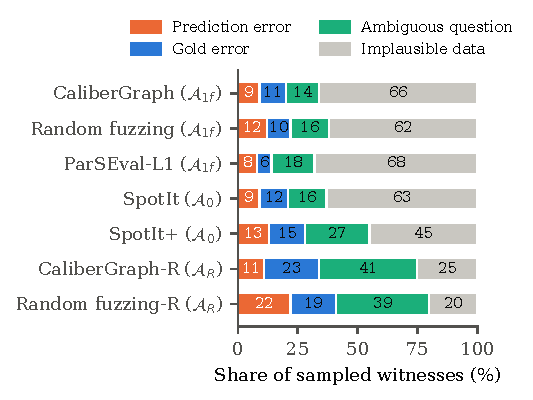
\includegraphics[width=\linewidth]{figs/attribution.pdf}
\caption{Attribution of random samples of 100 witnesses per tool (LLM annotation: two tool-blind passes, adjudicated). Upper five bars: first-stage tools at $\mathcal A_{1f}$ (SpotIt and SpotIt+ at $\mathcal A_0$); lower two: second-stage tools at $\mathcal A_R$.}\label{fig:attribution}
\end{figure}

The two annotation passes agree on \V{attrAgree}\,\% of the \V{attrN} first-stage witnesses ($\kappa=\V{attrKappa}$); \V{attrAdj} disagreements were adjudicated. For every tool, \V{attrImplMin}--\V{attrImplMax}\,\% of the sampled witnesses separate the queries only on implausible data, and only \V{attrErrMin}--\V{attrErrMax}\,\% expose an error of the prediction (Fig.~\ref{fig:attribution}; CaliberGraph: \V{pCGImpl}\,\% implausible, CI over questions \V{pCGImplClusterCI}). The decisive implausible facts are of few kinds: \texttt{NULL} in a column that is never \texttt{NULL} in BIRD; duplicates of what is unique in reality (a badge awarded twice, two races of one Grand Prix in a season); values that do not occur (a negative round, an atom identifier of the wrong pattern); and inconsistent records (a school whose county differs between two tables, a bond stored in one direction, an account without owner). Weighted by certified counts, CaliberGraph yields an estimated \V{estCGMeaningful} meaningful witnesses \V{estCGMeaningfulCI} and random fuzzing \V{estFZMeaningful} \V{estFZMeaningfulCI}: CaliberGraph's lead of \V{vsFZDiff} certified pairs over fuzzing does \emph{not} carry over to meaningful witnesses, and the estimated prediction errors its witnesses expose (\V{estCGErr}) are not more than fuzzing's (\V{estFZErr}). Of the \V{nSIClaims} pairs SpotIt claims to be non-equivalent, \V{nSILzero} can be re-certified, and an estimated \V{estSIErr} of these expose a prediction error. Since attribution judges the returned witness, not the pair, these are lower bounds on errors among certified pairs.

\textbf{Is the attribution valid? (Stage 3, pre-registered.)} Two human annotators labelled random samples of witnesses, half from each stage, independently and blind to tool, tier and AI verdict, in two rounds of \V{hvN} new witnesses each. In round~1 they saw only the witness and the queries: they agreed with each other on \V{hvAgreeHH} labels ($\kappa=\V{hvKappaHH}$; on implausible vs.\ other, $\kappa_2=\V{hvKappaHHbin}$) but not with the AI ($\kappa=\V{hvKappaHAmin}$--\V{hvKappaHAmax}), and each chose \emph{implausible data} only \V{hvHImpOne} times in 60 items, on different items, and \V{hvImpHOne} and \V{hvImpHTwo} times among the 30 first-stage witnesses, where the AI chose it \V{hvImpAIOne} times. Many of their reasons describe the anomaly the AI cites --- e.g., a lookup row \texttt{(3,'Bad')} where BIRD stores \texttt{(3,'Neutral')} --- but resolve it as an error of one query \emph{on the witness}. In round~2 every item also showed mechanically generated facts about $D_0$ (\texttt{NULL} counts, uniqueness and frequencies of the witness values of every referenced column), and the instructions asked first whether the difference could arise on real data. The annotators now chose \emph{implausible data} \V{hvTwoImpHOne} times each, agreed on it ($\kappa_2=\V{hvTwoKappaBin}$, CI \V{hvTwoKappaBinLo}--\V{hvTwoKappaBinHi}), and reproduced the difference between the tiers (\V{hvTwoImpConsOne} of the \V{hvTwoConsOne} first-stage and \V{hvTwoImpConsTwo} of the \V{hvTwoConsTwo} second-stage witnesses on which both agreed; one-sided Fisher $p=\V{hvTwoP}$), but agreed with the AI item by item only moderately ($\kappa_2=\V{hvTwoKappaAIbinMax}$, below the pre-registered 0.60). The shares we report in Fig.~\ref{fig:attribution} and below are the AI's and carry this uncertainty. ($\kappa_2$: Cohen's $\kappa$ on implausible vs.\ other.) Beyond implausibility, humans and AI also differ in the other labels (Table~\ref{tab:humanai}; five-label $\kappa$ \V{hvTwoKappaHAfiveMin}--\V{hvTwoKappaHAfiveMax} in round~2): the humans call many more witnesses prediction errors and almost none ambiguous, so every share of meaningful labels we report from the AI attribution should be read next to this table. A second model (Claude Sonnet~5.5) with the AI annotator's prompt and data access agreed with it on \V{cmN} witnesses ($\kappa=\V{cmKappaBin}$) and reproduced the drop between the stages (\V{cmImpOne} vs.\ \V{cmImpTwo} of 100).

\textbf{An annotator-free test (post hoc).} We repaired each first-stage witness locally, replacing the cells that violate the data profile $\Pi$ (Section~\ref{sec:profile}) by real values in 20 random repairs, and re-ran both queries. The difference vanished on every repair for \V{xVan} of \V{xN} witnesses (\V{xVanPct}\,\%) and survived on some for \V{xSurv}; it vanished for \V{xImpVanPct}\,\% of the witnesses the AI called implausible, but also for \V{xOthVanPct}\,\% of the others, and it vanished for \V{xHumVan} of the \V{xHumRep} repaired first-stage witnesses that both round-2 annotators called implausible. Yet for \V{xVanPairARpct}\,\% of the witnesses whose difference vanished (and \V{xPairARpct}\,\% of all), CaliberGraph-R or fuzzing-R found an $\mathcal A_R$ witness for the same pair: the two queries do differ on realistic data, but the first-stage witness does not show it. Without the facts, the round-1 annotators judged the \emph{pair} (which query answers the question); the AI, the round-2 annotators and the repair test judge the \emph{witness} (whether this database is evidence of that difference). The three are not independent of our definition: the facts shown in round~2 and the cells the repair replaces both come from $D_0$ and its profile, so they test the consistency of an operational notion of realism, not realism itself.


\subsection{RQ3: Data-grounded witnesses}\label{sec:rresults}

\begin{table}[t]
\centering\footnotesize
\caption{The data profile $\Pi$ mined from the eleven BIRD databases (75 tables, 3.9\,M rows; 258\,s on one core) and the share of first-stage $\mathcal A_{1f}$ witnesses (distinct EX-correct pairs) that violate each constraint class on the columns either query references (post hoc). CG: CaliberGraph; PSE: ParSEval-L1.}\label{tab:profile}
\setlength{\tabcolsep}{2pt}\scriptsize
\Tab{profile_icde}
\end{table}

None of CaliberGraph's \V{nCGLonef} first-stage witnesses satisfies the full data profile, and \V{nCGAtRq} satisfy it on the referenced columns. Column-level mined constraints do not close the gap: CaliberGraph+SC certifies \V{nCGSCLtwo} pairs at $\mathcal A_2$ but only \V{nCGSCAtR} at $\mathcal A_R$, none of SpotIt+'s \V{nSIPLtwo} $\mathcal A_2$ counterexamples reaches $\mathcal A_R$, and \V{pSIPImpl}\,\% of SpotIt+'s sampled witnesses are implausible. CaliberGraph-R certifies \V{nCGRAtR} EX-correct pairs (\V{pCGRAtR}\,\%) at $\mathcal A_R$, against \V{nFZRAtR} for random fuzzing-R with the same data access, repair and acceptance (difference \V{tCGRvsFZRRDiff}, CI \V{tCGRvsFZRRCI}); ParSEval-R certifies \V{ablRPV} of the \V{nSubR} subsample pairs, on which CaliberGraph-R certifies \V{ablRFull}. H5 is supported, and the lead holds on the schemas held out in the first stage, which informed the tier's design (\V{rateCGRHeld} vs \V{rateFZRHeld}\,\% of EX-correct pairs), as on the others (\V{rateCGROther} vs \V{rateFZROther}\,\%).

\textbf{Why schema-tier witnesses fail the profile (post hoc).} On the columns the queries reference (Table~\ref{tab:profile}), 72--86\,\% of the first-stage witnesses use a value outside the column's observed domain (an unseen category, shape or range), 30--70\,\% put a \texttt{NULL} into one of the 420 columns that are never \texttt{NULL} in BIRD, and 20--56\,\% break a value dependency (e.g., a county code paired with another county's name); half of ParSEval's minimal instances also duplicate a unique column combination. Every constraint class is violated by some tool's witnesses. Certified counts are insensitive to the categorical thresholds of the profile: re-certifying the stored witnesses with halved or doubled thresholds changes CaliberGraph-R's distinct certified pairs from \V{thrCGRFrozen} to \V{thrCGRLooser} or \V{thrCGRStricter}, fuzzing-R's from \V{thrFZRFrozen} to \V{thrFZRLooser} or \V{thrFZRStricter}, and admits none of CaliberGraph's first-stage witnesses.

\textbf{What the tier changes.} \V{pCGRImpl}\,\% of CaliberGraph-R's sampled witnesses rely on implausible data (CI over questions \V{pCGRImplClusterCI}), against \V{pCGImpl}\,\% of CaliberGraph's $\mathcal A_{1f}$ witnesses (H7; one-sided $p=\V{hSevenP}$, and $p\V{hSevenClusterP}$ over questions; pass agreement \V{attrRAgree}\,\%, $\kappa=\V{attrRKappa}$). The drop holds on the first-stage held-out schemas (\V{implCGRHeld} vs \V{implCGHeld}) and on the others (\V{implCGROther} vs \V{implCGOther}); fifty first-stage witnesses re-annotated in the same batch received the same verdict in \V{calibSame} cases, so it is not annotator drift. The rise in the meaningful share is due to the tier, not to the search: random fuzzing-R reaches \V{pFZRMeaningful}\,\%. CaliberGraph-R yields an estimated \V{estCGRMeaningful} meaningful witnesses against \V{estFZRMeaningful} for fuzzing-R; the difference (\V{hSixDiff}) was significant under the pre-registered parametric bootstrap (CI \V{hSixCI}, $p=\V{hSixP}$) but not robustly so under a bootstrap over questions (CI \V{hSixClusterCI}, one-sided $p=\V{hSixClusterP}$), so we regard H6 as only weakly supported. Post hoc, fuzzing-R's witnesses show a prediction error more often (estimated \V{estFZRErr} against \V{estCGRErr}); as its certified pairs are almost a subset of CaliberGraph-R's (\V{tCGRvsFZRRBOnly} exceptions), the difference lies in \emph{which} witness is returned for a pair.

\textbf{A limitation of the tier.} A sub-database may omit the entity a question names, so that one query returns no row and the other a row of \texttt{NULL}s; \V{nEmptyNullCGR} of CaliberGraph-R's and \V{nEmptyNullFZR} of fuzzing-R's 100 sampled witnesses are of this kind. Under $\mathcal C_{\mathrm{len}}$, which equates the two, CaliberGraph-R certifies \V{nCGRAtRClen} pairs and fuzzing-R \V{nFZRAtRClen}.

\textbf{A meaningful data-grounded witness.} For ``How many cards available in paper have a positive starting maximum hand size?'' the evidence defines availability as \texttt{LIKE '\%paper\%'}, but the gold query tests \texttt{availability = 'paper'}; CaliberGraph-R returns three real cards, one with the observed value \texttt{'arena,mtgo,paper'}, on which the gold query counts one card and the prediction two --- a gold query that contradicts its own evidence.

\textbf{Recall on known positives.} CaliberGraph finds an $\mathcal A_{1f}$ witness for \V{rCGLonef}\,\% of the \V{nExi} known positives, against \V{rPVLonef}\,\% for ParSEval-L1, \V{rFZLonef}\,\% for fuzzing and \V{rSI}\,\% claimed by SpotIt (H3). At $\mathcal A_R$ the figure is a sanity check rather than an estimate: $D_0$ itself separates every known positive and satisfies its profile up to the approximate cross-key rules, and CaliberGraph-R finds a witness for \V{rCGRAtR}\,\% (fuzzing-R \V{rFZRAtR}\,\%). No recall estimate exists for EX-correct pairs, on which a missed difference is invisible.


\subsection{RQ4: Effect on accuracy and rankings}\label{sec:rankings}

\begin{table}[t]
\centering\footnotesize
\caption{Per-system effect on the 1,174 test questions. Count-based: share of EX-correct predictions with a CaliberGraph $\mathcal A_{1f}$ witness, and EX after removing all of them (EX$'$). Error-weighted: certified share $\times$ attributed prediction-error rate (\V{errShareCG}\,\% at $\mathcal A_{1f}$, \V{errShareCGR}\,\% at $\mathcal A_R$), in points of EX; a lower bound (post hoc).}\label{tab:systems}
\setlength{\tabcolsep}{3pt}
\Tab{systems_icde}
\end{table}

Counting every $\mathcal A_{1f}$ witness as an error, \V{fpShareMin}--\V{fpShareMax}\,\% of each system's EX-correct predictions are removed, EX drops by \V{exDropMin}--\V{exDropMax} points and six to eight of the ten systems change rank, depending on how two exact EX ties are broken (Kendall's $\tau_b=\V{kendallTau}$; Table~\ref{tab:systems}); SpotIt's claims imply \V{ptsCountSpotItMin}--\V{ptsCountSpotItMax} points. RQ2 shows that most of these witnesses are not errors. Weighting each tool's certified share by its attributed prediction-error rate gives \V{ptsErrOnefMin}--\V{ptsErrOnefMax} points per system at $\mathcal A_{1f}$ and \V{ptsErrRMin}--\V{ptsErrRMax} at $\mathcal A_R$ (post hoc), with rankings unchanged except within the two exact ties ($\tau_b=\V{tauErrOnef}$ at both tiers); since one error rate is applied per tier, the rankings follow the certified shares, which differ little between systems. The estimates are lower bounds, since a pair whose returned witness is implausible may still be an error, and the error rate of each sample is uncertain (CaliberGraph-R: \V{errShareCGR}\,\%, interval over questions about 5--18\,\%). They also depend on who attributes: with the human annotators' pooled error rates (post hoc; \V{humErrPctOnef}\,\% of agreed schema-tier and \V{humErrPctR}\,\% of agreed $\mathcal A_R$ witnesses, Table~\ref{tab:humanai}), the same weighting gives \V{ptsHumOnefMin}--\V{ptsHumOnefMax} points at $\mathcal A_{1f}$ and \V{ptsHumRMin}--\V{ptsHumRMax} at $\mathcal A_R$, where counting every witness gives \V{ptsCountRMin}--\V{ptsCountRMax}. Data grounding thus changes what witnesses mean much more than how many errors they expose: the estimated prediction errors are similar at both tiers (\V{estCGErr} and \V{estCGRErr} for CaliberGraph and CaliberGraph-R). By the AI attribution, 58--64\,\% of the sampled $\mathcal A_R$ witnesses point to gold-query defects or ambiguities, some on sub-databases without the entity the question names; the human annotators disagree, attributing about half of the agreed $\mathcal A_R$ witnesses to prediction errors and almost none to ambiguity.


\subsection{RQ5: Ablation, cost and benchmark issues}\label{sec:ablation}

\begin{table}[t]
\centering\footnotesize
\caption{Ablation on a random subsample of \V{nSub} distinct EX-correct test pairs (5\,s per pair). Left: first stage, $\mathcal A_{1f}$ (H4). Right: second stage, $\mathcal A_R$, with baselines on the same subsample.}\label{tab:ablation}
\setlength{\tabcolsep}{3pt}
\begin{tabular}{@{}lrr@{}}
\toprule
Configuration & $\mathcal A_{1f}$ & $\Delta$\\
\midrule
CaliberGraph & \V{subFull} & \\
$-$anchoring & \V{subNoAnchor} & +1\\
$-$isolation & \V{subNoIso} & +2\\
$-$join graph & \V{subNoJoin} & $-$11\\
$-$SQLite domain & \V{subNoDomain} & +2\\
budget 10\,s & \V{subTen} & 0\\
ParSEval-L1 5\,s/10\,s & \multicolumn{2}{r}{\V{subPVFive}/\V{subPVTen}}\\
\bottomrule
\end{tabular}\hfill
\begin{tabular}{@{}lrr@{}}
\toprule
Configuration & $\mathcal A_R$ & $\Delta$\\
\midrule
CaliberGraph-R & \V{ablRFull} & \\
$-$real sub-DBs & \V{ablRNoReal} & $-$48\\
$-$synthesis & \V{ablRNoSyn} & $-$5\\
$-$anchoring & \V{ablRNoAnchor} & $-$11\\
$-$join completion & \V{ablRNoJoin} & $-$8\\
Random fuzzing-R & \V{ablRFuzz} & \\
ParSEval-R & \V{ablRPV} & \\
\bottomrule
\end{tabular}
\end{table}

\begin{figure}[t]
\centering
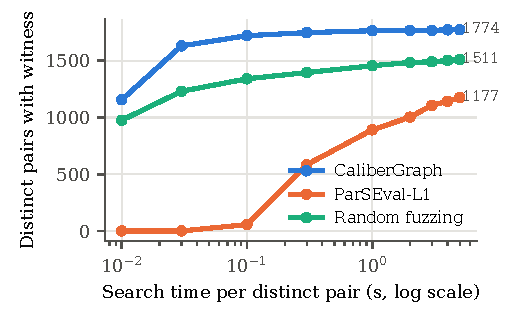
\includegraphics[width=0.92\linewidth]{figs/time_to_witness.pdf}
\caption{Distinct EX-correct pairs with a certified $\mathcal A_{1f}$ witness found within a given search time (first stage, 5\,s budget; a solver run that overruns the budget is not counted, so ParSEval-L1 reaches 1,177 of its 1,196 pairs).}\label{fig:time}
\end{figure}

In the first stage, join-graph completion is the only component whose removal lowers the count significantly (\V{hFourNoJoinFullOnly} of \V{subFull} pairs lost, none gained; Holm-adjusted $p=0.004$); removing anchoring, isolation or the SQLite value domain changes the count by at most two pairs, and the median time to a witness stays at 6--8\,ms. \textbf{H4 is not supported}: the differences these components target are also reached by the other phases and by the mutation loop, which applies the same operators at random, so their benefit on development pairs did not carry over. In the second stage, the real sub-database phase accounts for most witnesses (\V{ablRNoReal} without it, $p=\V{ablRNoRealP}$, fewer than fuzzing-R), and anchored retrieval ($p=\V{ablRNoAnchorP}$) and join completion ($p=\V{ablRNoJoinP}$) also contribute, whereas constrained synthesis adds few witnesses ($p=\V{ablRNoSynP}$).

\textbf{Cost.} When CaliberGraph finds an $\mathcal A_{1f}$ witness, the median search time is \V{tCGMedian}\,s (\V{tCGWithinOne}\,\% within 1\,s; Fig.~\ref{fig:time}); ParSEval-L1 needs \V{tPVMedian}\,s and CaliberGraph-R \V{tCGRRMedian}\,s at $\mathcal A_R$, including its queries to $D_0$. Most distinct pairs, however, end without a witness after the full budget, so the budget dominates the cost: auditing the accepted test predictions of one system (about 800) alone with CaliberGraph-R takes \V{costSysMean} core-hours on average (\V{costSysMin}--\V{costSysMax}), or 6.9 core-hours for all ten systems when identical predictions are shared. Doubling the budget leaves CaliberGraph's count unchanged and raises ParSEval-L1's from \V{subPVFive} to \V{subPVTen}; at $\mathcal A_R$ (post hoc, same subsample) it changes CaliberGraph-R's count from 195 to 193 and fuzzing-R's from 151 to 153, so neither stage is budget-bound. Mining the profile is a one-time cost per benchmark (Section~\ref{sec:profile}). Attribution, which F2 (Table~\ref{tab:findings}) makes necessary, is a manual or model-assisted cost of a sample per tool and is not included.

\textbf{Root causes and benchmark issues.} In a sample of 100 first-stage CaliberGraph witnesses, AI-annotated in two passes, \texttt{NULL} handling (30\,\%), filter predicates (18\,\%) and join paths (17\,\%) cause two thirds of the differences, followed by ordering and \texttt{LIMIT} ties (12\,\%), duplicates (9\,\%) and aggregates over empty input (8\,\%). Across all attribution samples (77 items from schema-tier samples, 46 from $\mathcal A_R$ samples), \V{nIssues} distinct test questions received a witness that the AI annotators judged to expose a gold-query defect (\V{nIssuesGold}) or an ambiguous question (\V{nIssuesAmb}). \V{nIssuesFragile} of them are fragile: their witness lacks the entity the question names, or the two results differ only in rounding or letter case; the remaining \V{nIssuesRobust} comprise \V{nIssuesRobustGold} gold defects and \V{nIssuesRobustAmb} ambiguities. The gold defects are \emph{latent}: on $D_0$ the gold query returns the accepted answer, but on the witness it answers the question wrongly. Recurrent kinds are wrong join paths or attributes (11), filters that contradict the question's evidence (8: inclusive \texttt{BETWEEN} for strict bounds, equality for \texttt{LIKE}, case-sensitive matches), aggregates over an empty selection that return \texttt{NULL} where a count of zero is meant (7), counts of rows or names where entities are counted (7), and averages that count \texttt{NULL}s (3); about half of the ambiguities concern ties. We release the list, with one witness, the annotators' reasons and these flags per question, as a candidate list for maintainers rather than a verdict. The list overlaps only weakly with the corrected annotations of Jin et al.~\cite{jin2026annotation} (pre-registered): of the \V{arcG} questions we flag as gold defects that their Arcwise-Plat set covers, \V{arcGk} (\V{arcGpct}\,\%) received a gold query with a different result on $D_0$, against \V{arcNpct}\,\% of the \V{arcNN} unflagged test questions (one-sided Fisher $p=\V{arcPone}$); our ambiguity flags do not predict their edits (\V{arcApct}\,\% vs.\ \V{arcANpct}\,\%). Counting textual corrections of the gold query, which our witnesses can expose although the corrected query returns the same result on $D_0$, the rate is \V{arcGtextPct}\,\% against \V{arcNtextPct}\,\% (post hoc). \V{arcGuntouched} flagged gold defects and \V{arcAuntouched} flagged ambiguities were left entirely unchanged by Arcwise-Plat.


\subsection{RQ6: Replication on Spider and on new systems (Stage 3)}\label{sec:replication}
We re-ran the frozen code on Spider~1.0 dev~\cite{yu2018spider}, which no design decision had seen: 20 databases (\V{spTables} tables, \V{spRows}\,k rows), 1,034 questions and six public prediction sets (DAIL-SQL~\cite{gao2024dailsql} with and without self-consistency, Graphix-T5~\cite{li2023graphix}, DIN-SQL~\cite{pourreza2023dinsql}, GPT-4 few- and zero-shot), i.e., \V{spN} EX-correct pairs. The pattern of the tiers replicates: CaliberGraph certifies \V{spCG} pairs at $\mathcal A_{1f}$ but \V{spCGR} at $\mathcal A_R$, fuzzing \V{spFZ} and \V{spFZR}. The search does not: CaliberGraph-R and fuzzing-R certify \V{spRCG} and \V{spRFZ} pairs at $\mathcal A_R$ (\V{spSOneA} vs.\ \V{spSOneB} discordant; one-sided $p=\V{spSOneP}$, CI over questions \V{spSOneLo} to \V{spSOneHi}; pre-registered S1 not supported), with equal recall on known positives (\V{spRecCGR} vs.\ \V{spRecFZR}\,\%). The attribution (two passes, $\kappa=\V{spKappa}$) finds \V{spImpCG} of \V{spNCG} sampled CaliberGraph witnesses implausible at $\mathcal A_{1f}$ against \V{spImpCGR} of \V{spNCGR} CaliberGraph-R witnesses at $\mathcal A_R$ (one-sided Fisher $p=\V{spSTwoP}$, not significant after Holm correction over the Stage-3 family) and none of \V{spNFZR} fuzzing-R witnesses; the estimated meaningful $\mathcal A_R$ witnesses are \V{spEstCGR} for CaliberGraph-R and \V{spEstFZR} for fuzzing-R (pre-registered S3 reversed: the difference has CI \V{spSThreeLo} to \V{spSThreeHi}, in fuzzing-R's favour). Post hoc, the implausible CaliberGraph-R witnesses almost all duplicate a real entity under a fresh key (two identical teachers), which the Spider profile does not forbid: on small tables our miner keeps only \V{spUcc} unique column combinations (BIRD: \V{bdUcc}), and \V{spCatShare}\,\% of the columns are categorical (BIRD: \V{bdCatShare}\,\%), so every admissible witness is close to a real sub-database and random real rows suffice.

On BIRD, the result of the search does replicate on systems the study had not seen: for the thirteen public prediction sets of BIRD Mini-Dev (GPT-3.5/4/4o, Llama-3, Mixtral, Phi-3), restricted to held-out test questions and to (question, prediction) pairs not seen before, CaliberGraph-R certifies \V{mdCGR} of \V{mdN} new EX-correct pairs at $\mathcal A_R$ and fuzzing-R \V{mdFZR} (\V{mdA} vs.\ \V{mdB} discordant; CI over questions \V{mdLo}--\V{mdHi}; Holm-adjusted $p$ \V{holmEOne}). Of \V{mdAttrN} sampled CaliberGraph-R witnesses, \V{mdImp} were attributed to implausible data, close to the second-stage share (\V{pCGRImpl}\,\%), and \V{mdErr} to a prediction error.

